\section{Règles}
\label{section:regles}
	Ce jeu SmallWorld, à la croisée entre le jeu de plateau SmallWorld et le jeu vidéo Civilization, est un jeu en tour par tour pour deux joueurs.
	L'objectif est bien entendu de gagner, au détriment de l'autre protagoniste. 

	La partie prend place sur un plateau à cases hexagonales, où chaque joueurs incarnera une faction différente.
	Possédants chacun un nombre d'unités de départ, ils pourront les déplacer à travers le plateau, afin de gagner des points d'occupation, ou des points de victoire.
	Lorsqu'un des joueurs ne possède plus d'unités en vie, la partie prends fin, et le joueur possédant le plus de points remporte la victoire.

	\subsection{Le plateau}
		Le plateau est composé de cases hexagonales, pouvant être de quatres types de terrains différents. Les cases et leurs textures sont illustrées en Figures \ref{fig:desert}, \ref{fig:moutain}, \ref{fig:field} et \ref{fig:forest}.

		\begin{figure}[h!]
			\centering
			
\includegraphics{figure/desert.png}
			\caption{Désert}
			\label{fig:desert}
		\end{figure}
		\begin{figure}[h!]
			\centering
			
\includegraphics{figure/moutain.png}
			\caption{Montagne}
			\label{fig:moutain}
		\end{figure}
		\begin{figure}[h!]
			\centering
			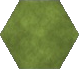
\includegraphics{figure/field.png}
			\caption{Plaine}
			\label{fig:field}
		\end{figure}
		\begin{figure}[h!]
			\centering
			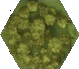
\includegraphics{figure/forest.png}
			\caption{Forêt}
			\label{fig:forest}
		\end{figure}

	\subsection{Les factions}
		Il existe actuellement trois factions: les nains (Figure \ref{fig:dwarf}), les elfes(Figure \ref{fig:elf}) et les orcs(Figure \ref{fig:orc}).

		\begin{figure}[h!]
			\centering
			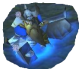
\includegraphics{figure/dwarf.png}
			\caption{Muradin, roi de la montagne.}
			\label{fig:dwarf}
		\end{figure}	
		\begin{figure}[h!]
			\centering
			
\includegraphics{figure/elf.png}
			\caption{Tyrande, elfe peu commode.}
			\label{fig:elf}
		\end{figure}		
		\begin{figure}[h!]
			\centering
			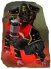
\includegraphics{figure/orc.png}
			\caption{Thrall, orc bagarreur.}
			\label{fig:orc}
		\end{figure}		
	
	\subsection{Début de partie}
		Les unités des joueurs sont placées à des coins opposés de la carte en début de partie, comme illustré en figure \ref{fig:debut_partie}.

		\begin{figure}[h]
			\centering
			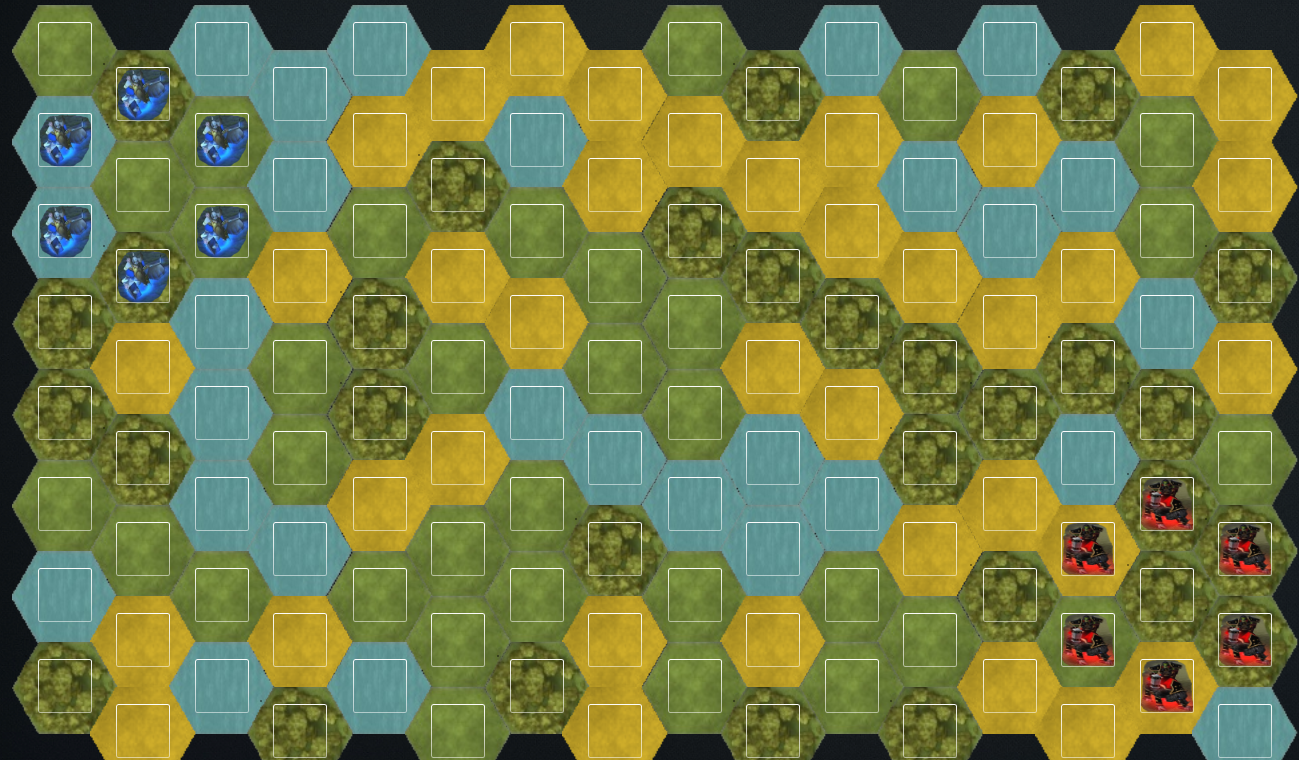
\includegraphics[width=1\textwidth]{figure/debut_partie.png}
			\caption{La distance séparant les joueurs en début de partie leur permettra d'avoir le temps d'établir une stratégie.}
			\label{fig:debut_partie}
		\end{figure}

	\subsection{Les déplacements}
		\`A chaque début de tour, les unités auront leurs points de déplacement réinitialisés à leur valeur par défaut ; 4.

		Un déplacement standard coûte 2 points, et ne peut s'effectuer uniquement vers une case adjacente à la case actuelle. Toutefois, afin de distinguer les factions entre elle, chaque faction possède un type de terrain \og préféré \fg. Il s'agit de la montagne pour les nains, de la forêt pour les elfes et du désert pour les orcs.

		Ainsi, lorsqu'une unité voudra se déplacer vers son type de terrain favori, le déplacement ne lui coûtera seulement un seul point.

		Par ailleurs, afin de pimenter le jeu, les nains possèdent une capacité de tunnels sous la montagne: un nain positionné sur une montagne pourra se déplacer vers n'importe quelle autre montagne de la carte, adjacente ou non. La seule condition est qu'il lui reste au moins un point de déplacement. Utiliser cette capacité consommera tout ses points de déplacement restants.

	\subsection{Les combats}
		Lorsque deux unités sont adjacentes, elles peuvent se bagarrer. Le système de combat, bien que très sommaire, est étudié afin de donner l'avantage aux jeux agressif, et ainsi éviter les parties passives.

		L'unité attaquante aura 66\% de chances de remporter la victoire. Par conséquent, l'unité se défendant a 34\% de chances de vaincre son assaillant. L'unité perdante sera détruite.

		Afin de pouvoir attaquer une unité, il faut avoir un minimum de deux points de déplacement. De plus, même en cas de victoire, tout les points de déplacement seront remis à 0.

	\subsection{Les points}
		Le but du jeu étant de faire un maximum de points, il convient maintenant d'expliquer comment les points sont calculés.

		A chaque fin de tour, chaque joueur se voit octroyé deux points par unité et par case occupée, et quatre si cette case est de son type favori.

		De plus, à chaque issue de combat, le possesseur de l'unité victorieuse se voit récompensé de 10 points.

	\subsection{Fin de partie}
		Lorsque l'un des joueurs ne possède plus d'unités, la partie se termine. Le joueur possédant le plus grand score remporte la victoire.

		Un écran affiche le nom du joueur victorieux, et un grand banquet est organisé en son honneur.

	Maintenant que les règles ont été définies, il est temps de montrer comment lancer une partie.